\documentclass{report}
\usepackage{graphicx} % Required for inserting images
\usepackage{geometry}
\usepackage{amsmath}
\usepackage{mathtools}
\usepackage{amssymb}
\usepackage{kotex}
\usepackage{makecell}
\usepackage{bytefield}
\usepackage{listings}
\usepackage{caption}
\usepackage{subcaption}

\captionsetup{labelformat=empty,labelsep=none,font=small}
\lstset{
    basicstyle=\small\ttfamily,
    commentstyle=\small\ttfamily,
    numbers=left,
    columns=flexible,
    breaklines=true,
    captionpos=b,
    xleftmargin=5.0ex,
    aboveskip=1.0em,
}

\title{CSED551 PA\#5 \\[0.5ex] {\normalsize :Deconvolution}}
\author{\small{20220848 Minsu Sun}}
\date{\small{December 20, 2024}}

\begin{document}

\maketitle

\section*{Code}

이번 Deconvolution을 구현하는 과정에서 사용된 함수의 설명이다.

\subsection*{Wiener Deconvolution}

\begin{lstlisting}[language=Python, caption=wiener\_deconv, firstnumber=179]
def wiener_deconv(b: np.ndarray, k: np.ndarray, c: float):
    blurred_img = b.astype(np.float32) / 255
    kernel = k.astype(np.float32) / np.sum(k)

    result = np.zeros_like(b).astype(np.float32)

    F_k = psf2otf(kernel, blurred_img.shape[:2])  # Degradation Function

    for idx in range(blurred_img.shape[2]):
        F_b = fft2(blurred_img[:, :, idx])
        F_l = (
            (F_k**2 / (F_k**2 + c)) * F_b / F_k
        )  # Wiener Deconvolution Formula: Minimum MSE Filter
        result[:, :, idx] = np.real(ifft2(F_l)) * 255

    return np.clip(result, 0, 255)
\end{lstlisting}

위 코드는 주어진 blurred image와 kernel을 이용하여 Wiener Deconvolution을 진행한다.
Wiener Deconvolution의 식에 따라 Frequency 도메인에서 blur된 이미지와 커널 필터 이미지를 이용해 deconvolution을 진행한다.

\subsection*{TV Deconvolution}

다음은 예제로 주어진 \code{demo\_L2.py}에서 가져온 코드 중 수정한 부분이다.

\begin{lstlisting}[language=Python, caption=Modified Code, firstnumber=90]
def deconv_L2(
    blurred: np.ndarray,
    latent0: np.ndarray,
    psf: np.ndarray,
    reg_strength: float,
    tau: float,
) -> np.ndarray:
    """
    Perform non-blind deconvolution using an L2 norm on the image gradient.

    Parameters:
    blurred (np.ndarray): The blurred image.
    latent0 (np.ndarray): Initial solution for the latent image.
    psf (np.ndarray): Blur kernel (point spread function).
    reg_strength (float): Regularization strength.
    weight_x (np.ndarray): Weight map for the x-direction gradient.
    weight_y (np.ndarray): Weight map for the y-direction gradient.

    Returns:
    np.ndarray: The deblurred image.
    """
    img_size = blurred.shape

    # Image gradient filters
    dxf = np.array([[0, -1, 1]])
    dyf = np.array([[0], [-1], [1]])

    latent = latent0.copy()

    # Compute the conjugate of the PSF by flipping it upside-down and left-and-right
    psf_conj = np.flip(psf)

    # compute b by convoling the blurred image with the conjugate PSF
    # K^T \cdot b
    b = fftconv2(blurred, psf_conj)
    b = b.ravel()

    # set x as the raveled latent image
    x = latent.ravel()

    # Parameters for the conjugate gradient method
    cg_param: Dict[str, np.ndarray] = {
        "psf": psf,
        "psf_conj": psf_conj,
        "img_size": img_size,
        "reg_strength": reg_strength,
        "dxf": dxf,
        "dyf": dyf,
        "tau": tau,
    }

    # Run the conjugate gradient method
    x = conjgrad(x, b, 25, 1e-4, Ax, cg_param)

    # Reshape the solution back to the original image size
    latent = x.reshape(img_size)
    return latent


def Ax(x: np.ndarray, p: Dict[str, np.ndarray]) -> np.ndarray:
    """
    Matrix-vector multiplication used in the conjugate gradient method.

    Parameters:
    x (np.ndarray): Input vector.
    p (Dict[str, np.ndarray]): Parameters containing PSF, weights, and gradients.

    Returns:
    np.ndarray: Result of the multiplication.
    """
    x = x.reshape(p["img_size"])
    # Convolve with PSF and its conjugate
    y = fftconv2(fftconv2(x, p["psf"]), p["psf_conj"])

    W_x = correlate(x, p["dxf"], mode="wrap")
    W_x = 1 / np.vectorize(lambda x: max(x, p["tau"]))(np.abs(W_x))
    W_y = correlate(x, p["dyf"], mode="wrap")
    W_y = 1 / np.vectorize(lambda x: max(x, p["tau"]))(np.abs(W_y))

    y += p["reg_strength"] * convolve(
        W_x * correlate(x, p["dxf"], mode="wrap"), p["dxf"], mode="wrap"
    )
    y += p["reg_strength"] * convolve(
        W_y * correlate(x, p["dyf"], mode="wrap"), p["dyf"], mode="wrap"
    )

    return y.ravel()
\end{lstlisting}

Iterative Re\-weighted Least Squares 방법을 적용하기 위해 Weight 계산을 진행하도록 수정하였다.
$Ax=b$의 형태를 가지도록 하여 Sample Code에서 제공한 Gradient Conjugate Solver를 사용하도록 하였다.
\code{cg\_param}으로 넘겨주던 고정된 Weight가 아닌 매번 iteration마다 이를 계산하여 사용한다.
Weight를 설정할 때 필요한 $\tau$ 또한 추가하여 이를 기반으로 $W_{x,y}$ 행렬을 구성하도록 하였다.
(원래의 IRLS 방법은 HW x HW Matrix를 사용하여 $W_{x,y}$를 나타내지만, 메모리 제한으로 인해 
H x W Matrix로 나타내어 Sparse한 Matrix를 Dense하게 사용하였다.)

다음은 위의 수정된 함수들을 이용하여 TV Deconvolution을 진행하는 함수이다.

\begin{lstlisting}[language=Python, caption=TV\_deconv, firstnumber=197]
def TV_deconv(b, k, tol=0.001, tau=1e-4):
    blurred_img = b.astype(np.float32) / 255
    kernel = k.astype(np.float32) / np.sum(k)

    result = np.zeros_like(b)

    for idx in range(blurred_img.shape[2]):
        img = blurred_img[:, :, idx]
        result[:, :, idx] = (
            deconv_L2(img, img, kernel, tol, tau) * 255
        )  # fix tau for typical 1e-4
    return np.clip(result, 0, 255)
\end{lstlisting}

주어진 RGB 채널을 각 채널로 분리하여 Deconvolution을 적용한 이후 다시 합쳐 이미지를 구성하였다.
IRLS 방법을 위한 $\tau$ 또한 같이 전달할 수 있도록 수정하였다.

\section*{Discussion - Wiener Deconvolution}

\subsection*{Parameter $c$}

Wiener Deconvolution의 목표는 아래와 같다. (Frequency Domain)

\begin{align*}
    \mathop{\min}\limits_{H} E[\Vert L-HB \Vert ^2]
\end{align*}

이는 아래와 같이 풀어 Error가 Minimum이 되는 Deconvolution Filter H를 얻는 것을 목표로 한다. (B: Blurred Image, L: Latent Sharp Image)

\begin{align*}
    B &= KL + N, \\ 
    \mathop{\min}\limits_{H} E[\Vert L-H(KL+N) \Vert] &= \mathop{\min}\limits_{H} E[\Vert (1-HK)L-HN \Vert] \\
    \mathop{\min}\limits_{H} E[\Vert (1-HK)L-HN \Vert] &=
    \mathop{\min}\limits_{H} \{\Vert 1-HK \Vert ^2 E[\Vert L \Vert ^2]-2(1-HK)E[LN] + \Vert H \Vert ^2 E[\Vert N \Vert ^ 2]\}
\end{align*}

우리는 Noise $N$을 평균이 0인 Normal Distribution을 따를 것으로 예상함으로, $L$과는 독립적이기에 $E[LN]=E[L]E[N]$이다.
평균을 0으로 가정하므로 $E[L]E[N]$는 결국 0이 된다. 이를 정리하면 아래와 같다.

\begin{align*}
    \mathop{\min}\limits_{H} \{\Vert 1-HK \Vert ^2 E[\Vert L \Vert ^2] + \Vert H \Vert ^2 E[\Vert N \Vert ^ 2]\}
\end{align*}

위의 식을 $H$를 기준으로 미분하여 기울기가 0이 되는 지점을 찾으면 이곳이 최적의 $H$라는 것을 알 수 있다.
이를 다시 $H$로 정리하면 아래와 같다.

\begin{align*}
    \Rightarrow -2(1-HK)E[\Vert L \Vert ^ 2] + 2HE[\Vert N \Vert ^2]=0 \\
    \Rightarrow H = \frac{KE[\Vert L \Vert ^2]}{K^2E[\Vert L \Vert ^2]+ E[\Vert N \Vert ^2]} = \frac{K^2}{K^2+\frac{E[\Vert N \Vert ^2]}{E[\Vert L \Vert ^2]}} \times \frac{1}{K}
\end{align*}

$B$에 $H$를 곱해 아래와 $l$을 공식화할 수 있다. ($F$는 Fourier Transform, $F^{-1}$은 Inverse Fourier Transform을 의미한다.)

\begin{align*}
    l=F^{-1}(\frac{K^2}{K^2+\frac{E[\Vert N \Vert ^2]}{E[\Vert L \Vert ^2]}} \times \frac{B}{K})
\end{align*}

SNR는 $Var(\text{Noise})$와 $Var{\text{Signal}}$의 비율로 나타나므로 위의 식을 아래와 같이 SNR의 표현으로 나타낼 수 있다.

\begin{align*}
    l=F^{-1}(\frac{K^2}{K^2+\frac{1}{SNR(\omega)}} \times \frac{B}{K})
\end{align*}

SNR은 기존에 예측이 되어야 하는 값이지만, Natural Image의 경우 Signal의 Variance가 $\frac{1}{\omega^2}$로 Scaling되며, Noise의 경우에는 보통 White Noise로 Variance가 상수인 경향을 가진다.
이를 통해 SNR을 다음과 같이 예상할 수 있다.

\begin{align*}
    \sigma_S &= \frac{1}{\omega^2} \\
    \sigma_N(\omega)&=\textit{constant} \\
    SNR(\omega)&=\frac{1}{c\omega^2}
\end{align*}

이에 따라 Latent Image는 다음과 같이 나타낼 수 있다.

\begin{align*}
    l=F^{-1}(\frac{K^2}{K^2+c\omega^2} \times \frac{B}{K})
\end{align*}

이를 Spatial Domain에서의 Fourier Transform과 함께 나타내면 다음과 같이 나타낼 수 있다.

\begin{align*}
    l=F^{-1}(\frac{|F(k)|^2}{|F(k)|^2+c} \times \frac{F(b)}{F(k)})
\end{align*}

\textbf{결론적으로, Wiener Deconvolution에서의 상수 $c$는 SNR을 나타내는 상수로 사용됨을 확인할 수 있다.}

아래는 Wiener Deconvolution의 결과이다.

\begin{figure}[htbp]
    \centering
    \subfloat[]{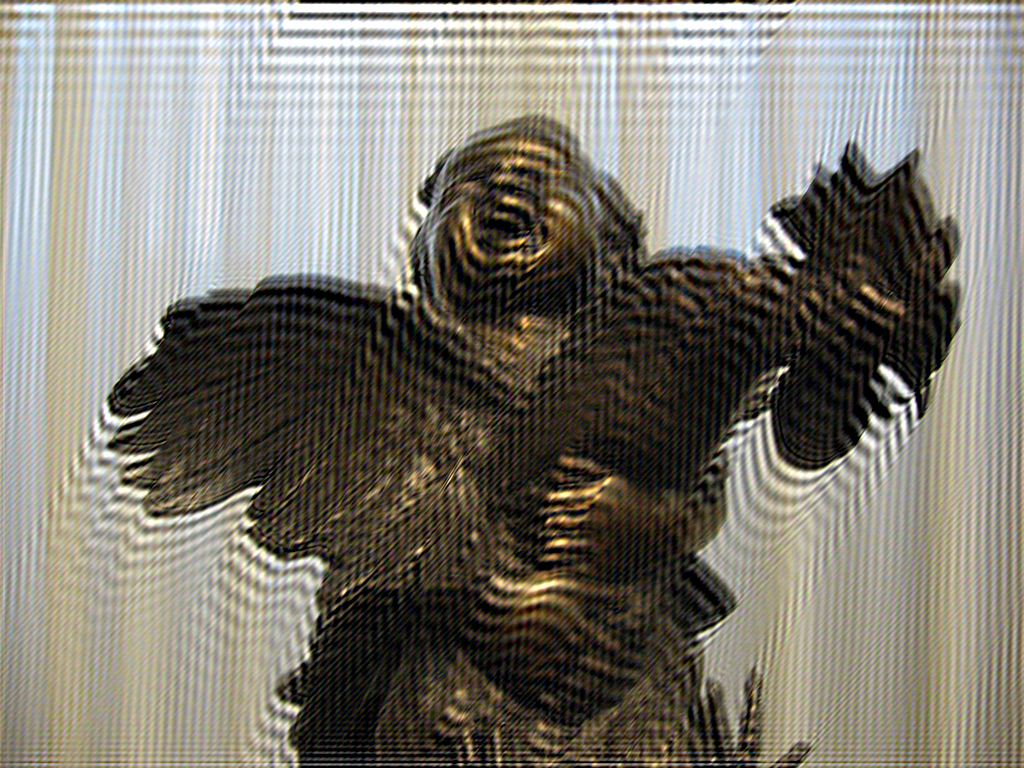
\includegraphics[width=0.2\linewidth]{../images/output/wiener/boy_statue_0.1.png}}
    \hspace{1pt}
    \subfloat[]{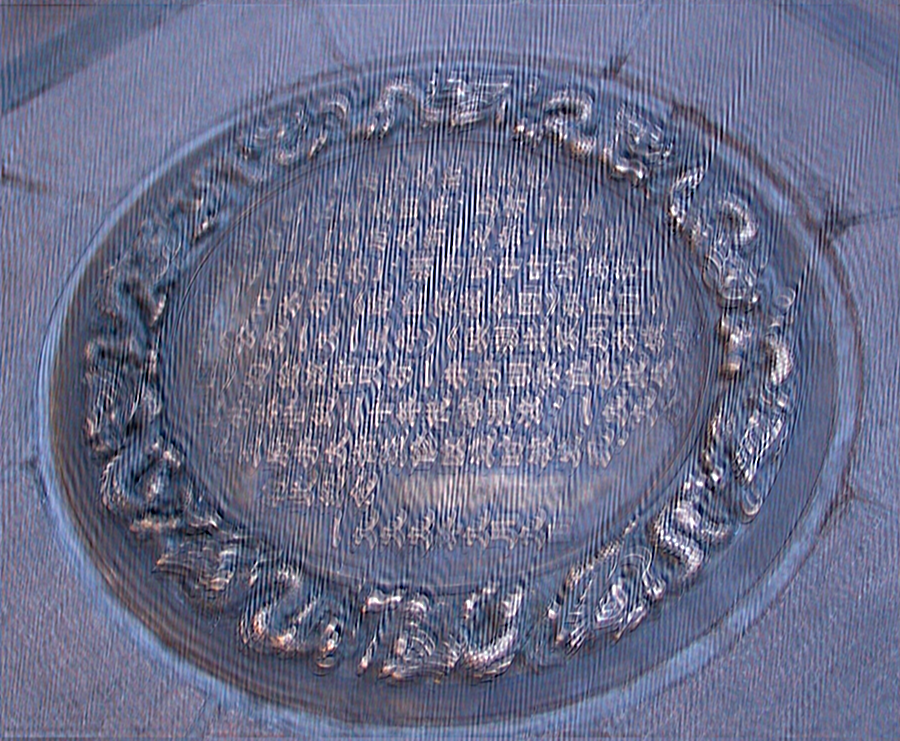
\includegraphics[width=0.2\linewidth]{../images/output/wiener/hanzi_0.1.png}}
    \hspace{1pt}
    \subfloat[]{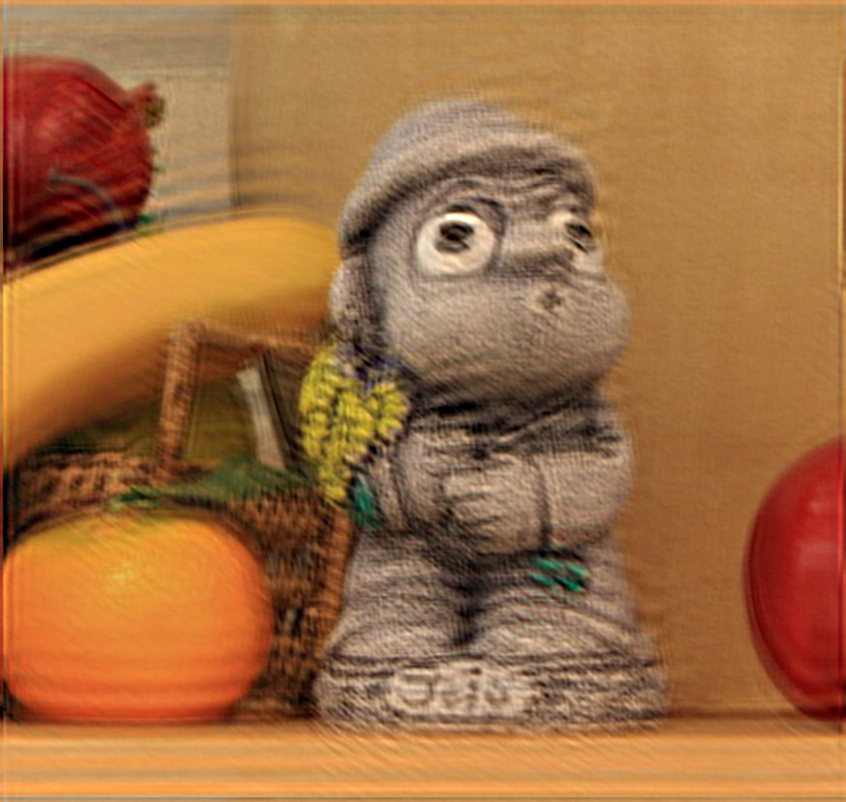
\includegraphics[width=0.2\linewidth]{../images/output/wiener/harubang_0.1.png}}
    \hspace{1pt}
    \subfloat[]{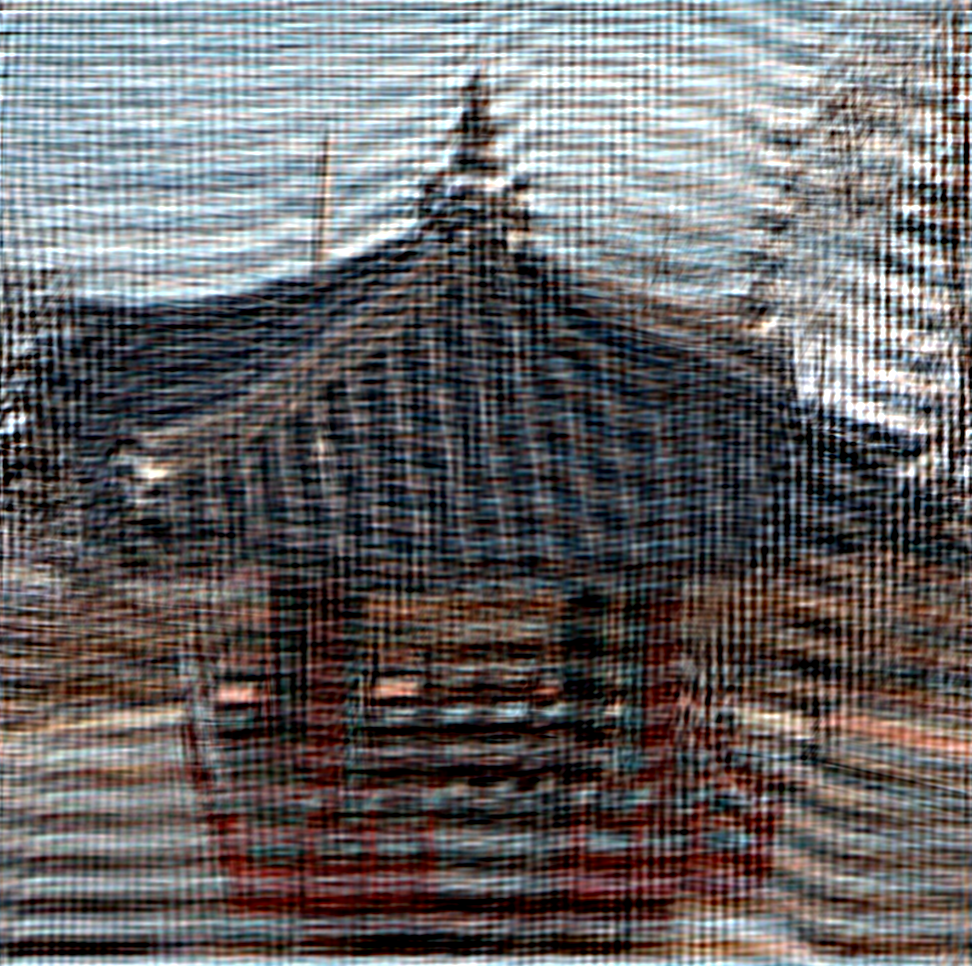
\includegraphics[width=0.2\linewidth]{../images/output/wiener/summerhouse_0.1.png}}
    \caption{Result of Wiener Deconvolution($c$=0.1)}
\end{figure}
\begin{figure}[htbp]
    \centering
    \subfloat[]{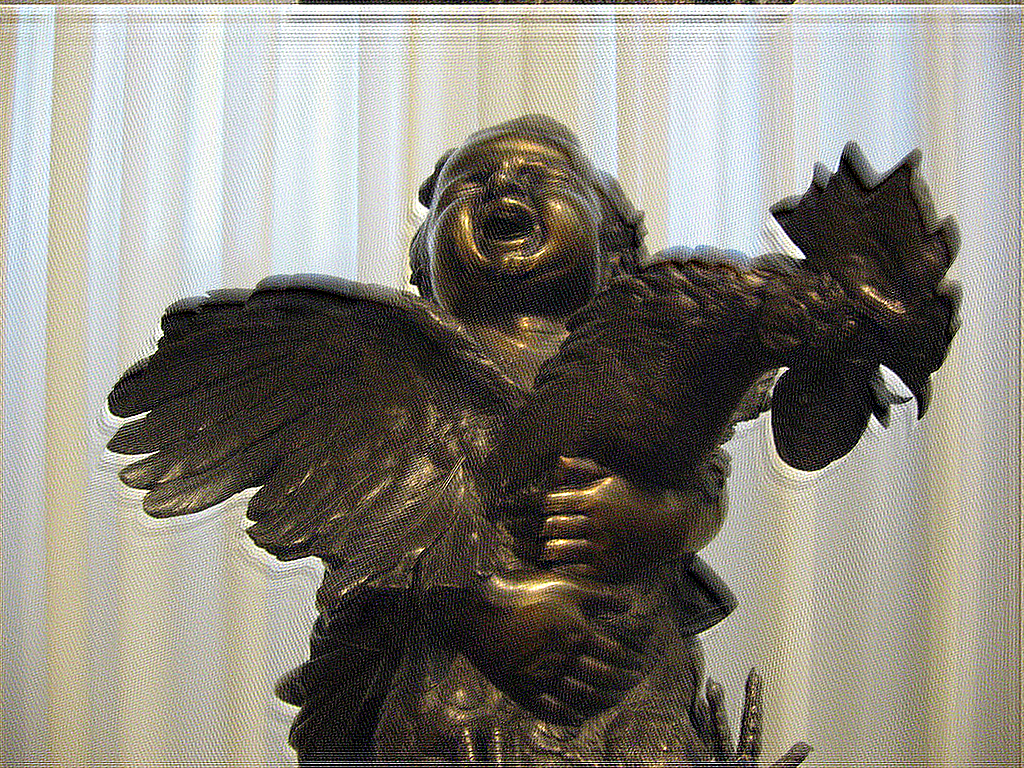
\includegraphics[width=0.2\linewidth]{../images/output/wiener/boy_statue_0.01.png}}
    \hspace{1pt}
    \subfloat[]{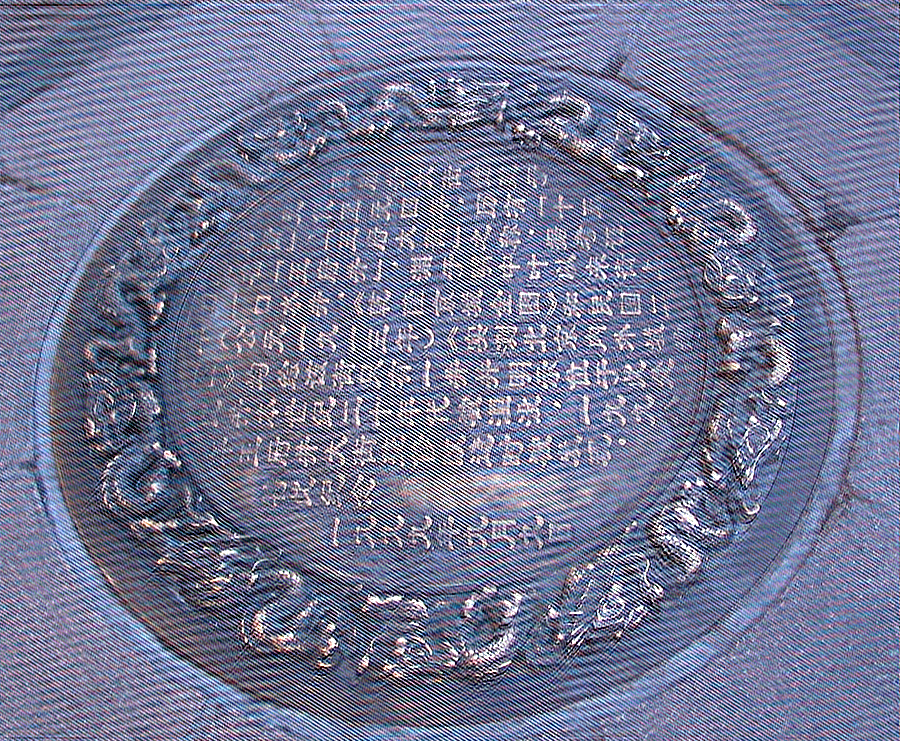
\includegraphics[width=0.2\linewidth]{../images/output/wiener/hanzi_0.01.png}}
    \hspace{1pt}
    \subfloat[]{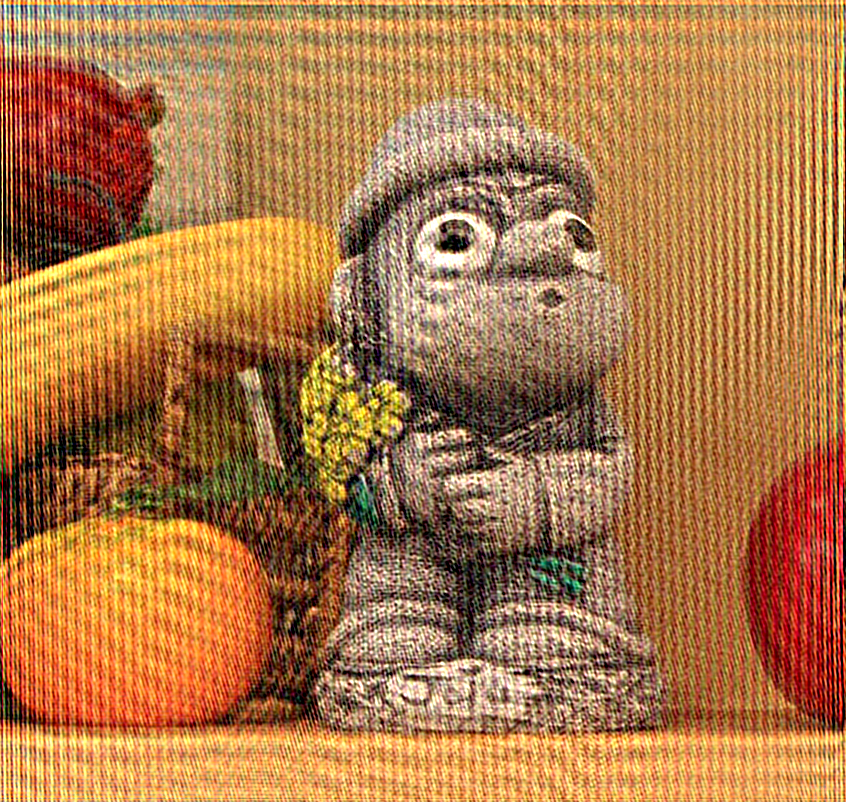
\includegraphics[width=0.2\linewidth]{../images/output/wiener/harubang_0.01.png}}
    \hspace{1pt}
    \subfloat[]{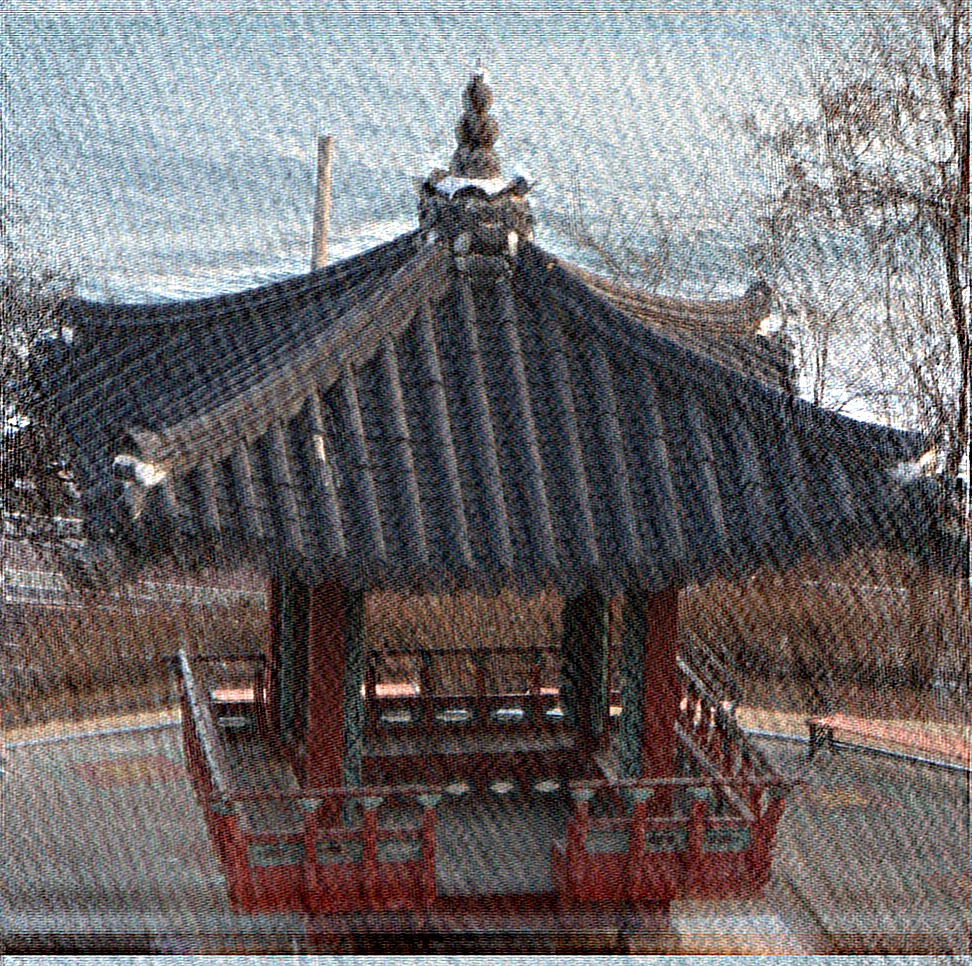
\includegraphics[width=0.2\linewidth]{../images/output/wiener/summerhouse_0.01.png}}
    \caption{Result of Wiener Deconvolution($c$=0.01)}
\end{figure}
\begin{figure}[htbp]
    \centering
    \subfloat[]{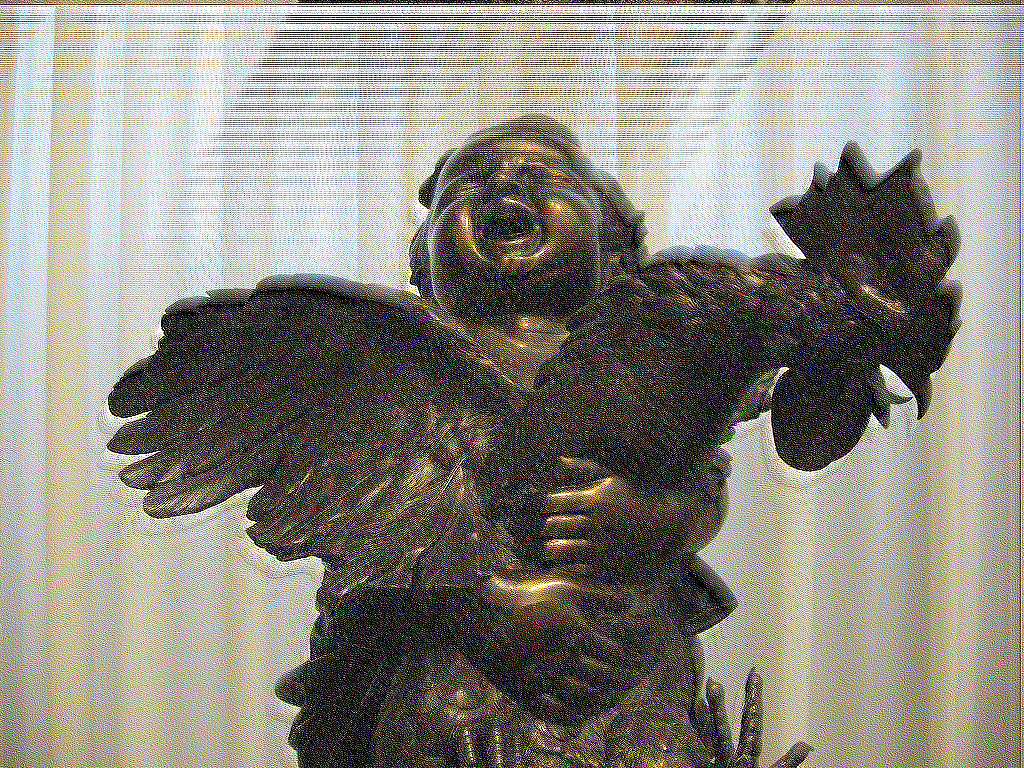
\includegraphics[width=0.2\linewidth]{../images/output/wiener/boy_statue_0.001.png}}
    \hspace{1pt}
    \subfloat[]{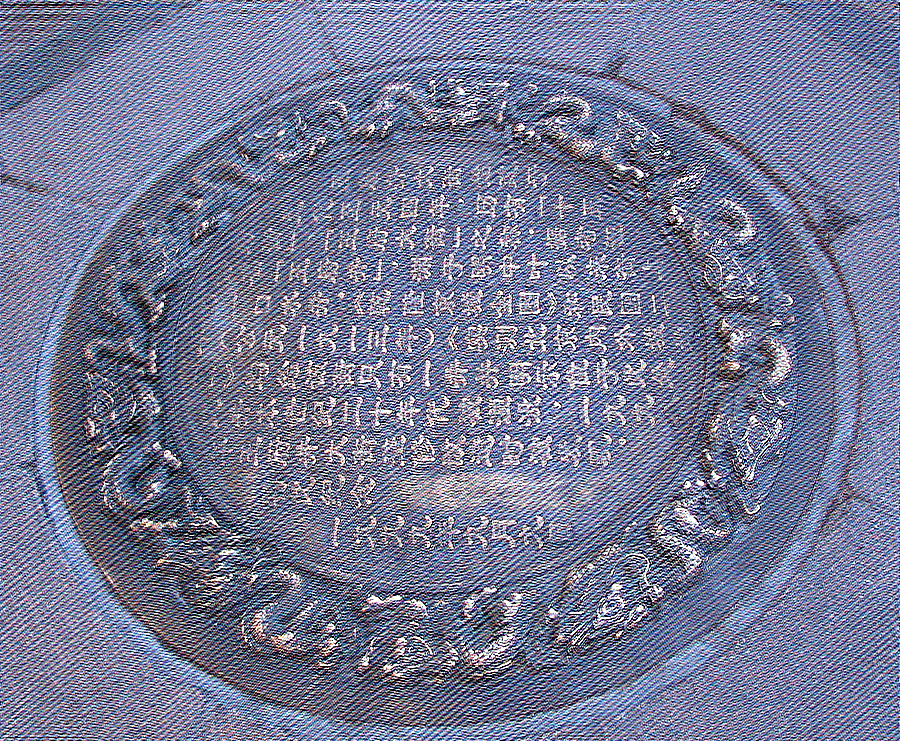
\includegraphics[width=0.2\linewidth]{../images/output/wiener/hanzi_0.001.png}}
    \hspace{1pt}
    \subfloat[]{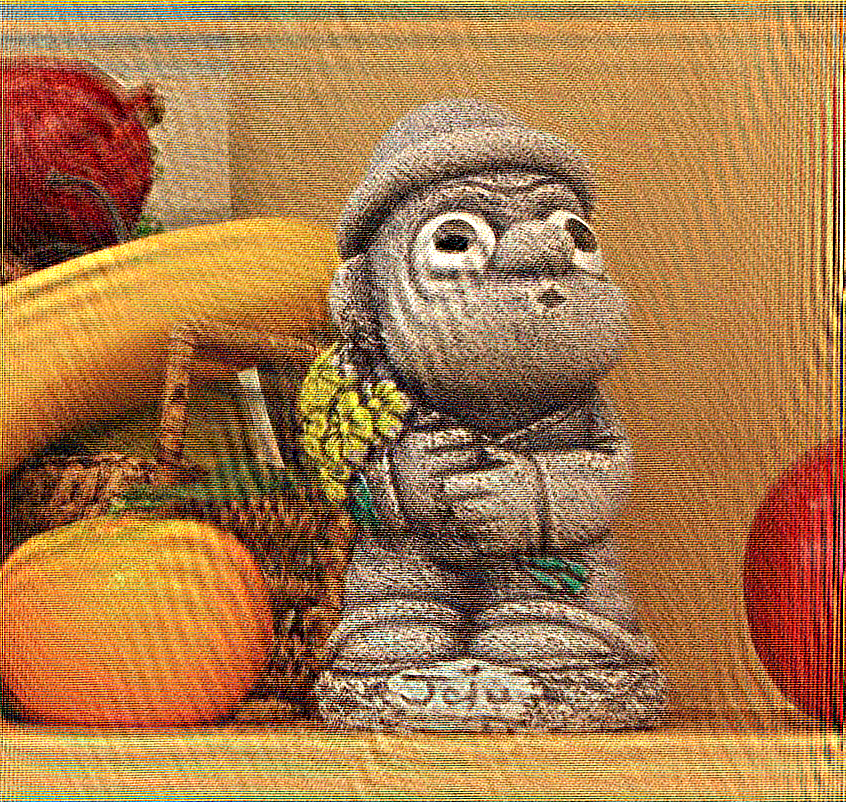
\includegraphics[width=0.2\linewidth]{../images/output/wiener/harubang_0.001.png}}
    \hspace{1pt}
    \subfloat[]{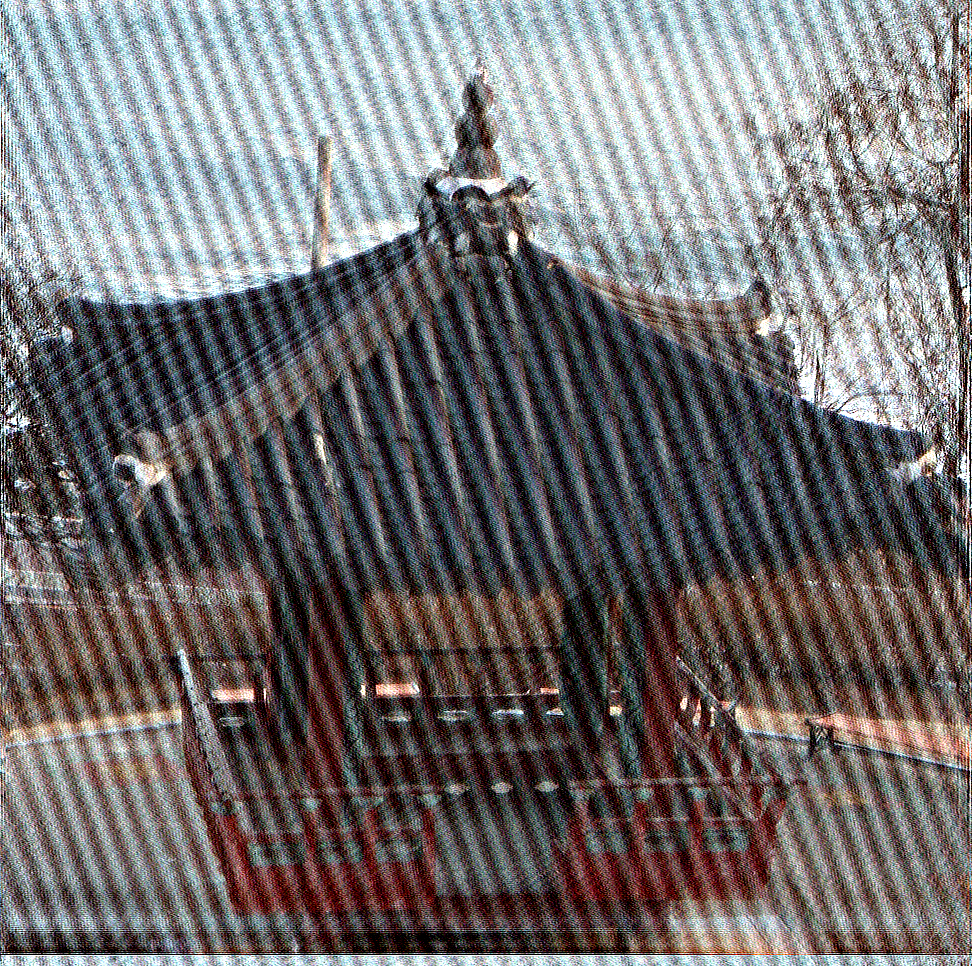
\includegraphics[width=0.2\linewidth]{../images/output/wiener/summerhouse_0.001.png}}
    \caption{Result of Wiener Deconvolution($c$=0.001)}
\end{figure}

Parameter $c$의 값에 따라서 결과가 달라지는 것을 볼 수 있다.

\subsection*{Limitation}

위의 정리에서 확인한 바와 같이, parameter $c$는 이미지의 SNR을 추정하는 값이다.
그렇기 때문에, 이미지마다 Noise의 정도를 생각하여 이를 결정해야 한다.
다만, 이에 대한 정보가 없을 경우 여러가지의 $c$ 값을 확인하여 결정해야 된다는 점이 한게점으로 생각된다.
결과에서도 확인할 수 있듯이, 특정 이미지에 특정 $c$ 값이 어올리는 것을 볼 수 있으며, 다른 이미지의 경우에는 다른 $c$ 값을 따르거나 혹은 아예 맞지 않을 수도 있다.
이미지의 Gradient 값을 이용해 SNR을 추정하여 이를 $c$의 값으로 결정하여 사용할 경우 더 나은 추정을 보일 것으로 생각된다.

\section*{Discussion - TV Deconvolution}

\subsection*{MAP Problem and Energy Function $E(l)$}

MAP 문제에 의하면 다음과 같은 목표를 가지고 문제를 풀도록 한다.

\begin{align*}
    l = \mathop{\max}\limits_{l} p(l | b, k)
\end{align*}

이는 posterior probability로 Bayes Theorem에 의하여 다음과 같이 나타낼 수 있다.

\begin{align*}
    l = \mathop{\max}\limits_{l} p(l | b, k) = \mathop{\max}\limits_{l} \frac{p(b | l, k)p(l)p(k)}{p(b)p(k)}
\end{align*}

이에 $-log$를 씌워 정리하면 다음과 같다.

\begin{align*}
    l &= \mathop{\max}\limits_{l} \frac{p(b | l, k)p(l)p(k)}{p(b)p(k)} \\
      &= \mathop{\min}\limits_{l} [-log(\frac{p(b | l, k)p(l)}{p(b)})] \\
      &= \mathop{\min}\limits_{l} [-log(p(b|l,k)) -log(p(l)) + log(p(b))] \\
\end{align*}

이 때, $p(b)$는 l에 따라 변화하지 않으므로 상수로 처리가능하며, $b=kl+n$이라는 Noise Model에 의해 다음과 같이 정리될 수 있다.

\begin{align*}
    l &= \mathop{\min}\limits_{l} [-log(p(b|l,k)) -log(p(l)) + log(p(b))] \\
      &= \mathop{\min}\limits_{l} [-log(p(b-kl|l,k)) -log(p(l)) + C] \\
      &(\because (b-kl) \sim \mathcal{N}(0,\sigma^2)) \\
      &= \mathop{\min}\limits_{l} [-log(N(b-kl|0,\sigma^2)) -log(p(l)) + C] \\
      &= \mathop{\min}\limits_{l} [C_1 \Vert b-kl \Vert ^2 -log(p(l)) + C] \\
      &= \mathop{\min}\limits_{l} [\Vert b-kl \Vert ^2 -log(p(l))]
\end{align*}

MAP의 목적은 에너지 함수를 최소화 시키는 것이므로, 위의 수식은 이에 따라 Latent $l$의 에너지 함수$E(l)$을 다음과 같이 정의할 수 있다.

\begin{align*}
    E(l) = \Vert b-kl \Vert ^2 -log(p(l))
\end{align*}

이 때, $l$의 prior $p(l)$을 다음과 같이 formulate 한다.

\begin{align*}
    p(l) = \frac{1}{Z}exp(-\frac{1}{\sigma_p^2}\sum_{x,y}\Vert \nabla f(x,y) \Vert)
\end{align*}

그럼 전체 에너지 함수 $E(l)$을 다음과 같이 정리할 수 있다.

\begin{align*}
    E(l) &= \Vert b-kl \Vert ^2 -log(p(l)) \\
         &= \Vert b-kl \Vert ^2 -log(\frac{1}{Z}exp(-\frac{1}{\sigma_p^2}\sum_{x,y}\Vert \nabla f(x,y) \Vert)) \\
         &= \Vert b-kl \Vert ^2 + \frac{1}{\sigma_p^2} \sum_{x,y}\Vert \nabla f(x,y) \Vert -log\frac{1}{Z}
\end{align*}

결국 MAP 문제의 목표 또한 다음과 같이 정리할 수 있다.

\begin{align*}
    l &= \mathop{\min}\limits_{l} [-log(p(b|l,k)) -log(p(l)) + log(p(b))] \\
      &= \mathop{\min}\limits_{l} [\Vert b-kl \Vert ^2 + \frac{1}{\sigma_p^2} \sum_{x,y}\Vert \nabla f(x,y) \Vert -log\frac{1}{Z}] \\
      &= \mathop{\min}\limits_{l} [\Vert b-kl \Vert ^2 + \alpha \sum_{x,y}\Vert \nabla f(x,y) \Vert]
\end{align*}

이는 결국 MSE 문제에서의 Regularization Term으로 $l$의 prior $p(l)$이 붙은 결과와 같다는 사실을 확인할 수 있다.
\textbf{$\alpha$를 통해 Regularization의 Preference를 조절하면서, 동시에 $l$의 prior $p(l)$의 분포를 예측하는 것과 같다.}

아래는 다양한 $\alpha$ 값에 따른 TV Deconvolution의 결과이다.

\begin{figure}[htbp]
    \centering
    \subfloat[]{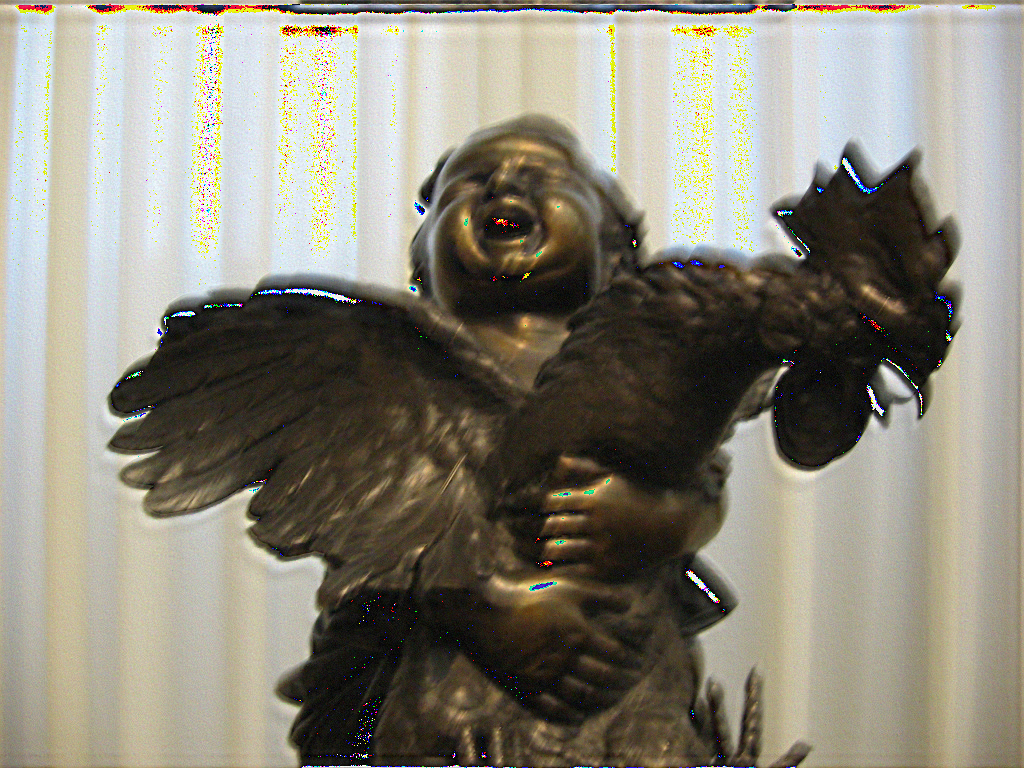
\includegraphics[width=0.2\linewidth]{../images/output/TV/boy_statue_0.01.png}}
    \hspace{1pt}
    \subfloat[]{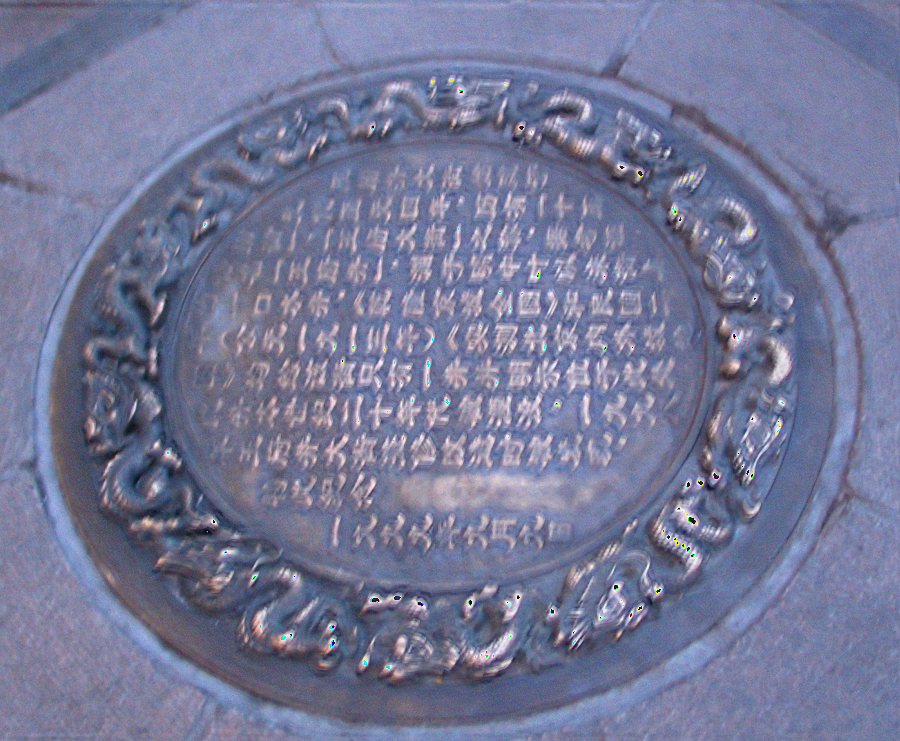
\includegraphics[width=0.2\linewidth]{../images/output/TV/hanzi_0.01.png}}
    \hspace{1pt}
    \subfloat[]{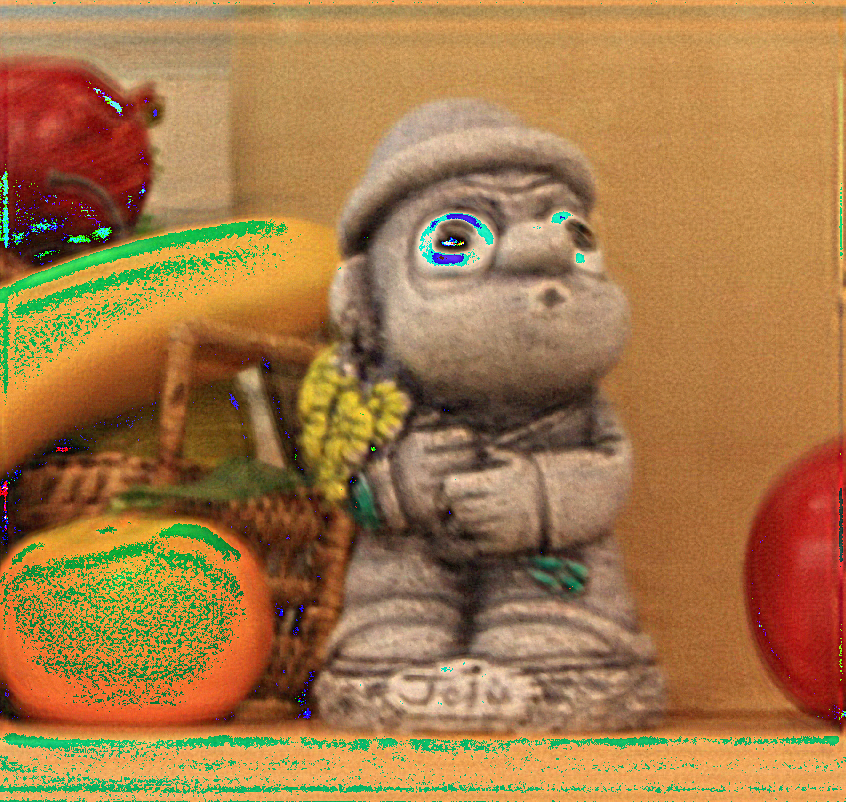
\includegraphics[width=0.2\linewidth]{../images/output/TV/harubang_0.01.png}}
    \hspace{1pt}
    \subfloat[]{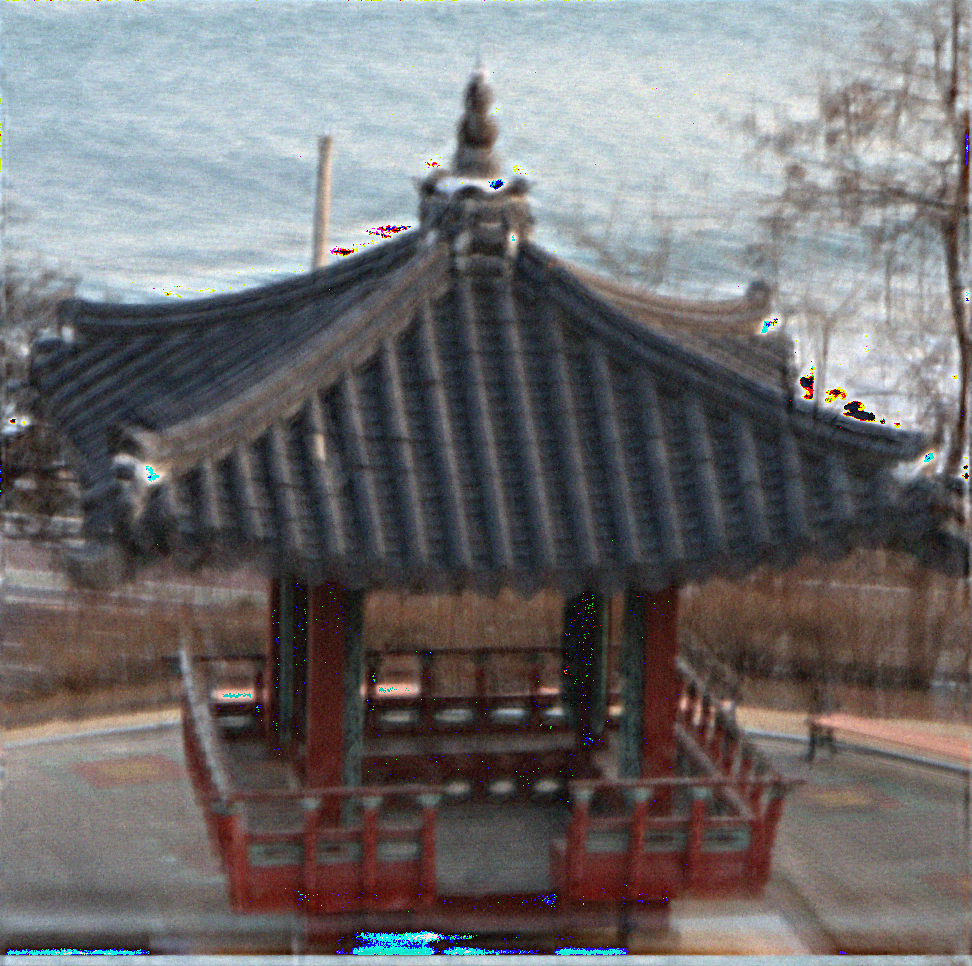
\includegraphics[width=0.2\linewidth]{../images/output/TV/summerhouse_0.01.png}}
    \caption{Result of TV Deconvolution($c$=0.10)}
\end{figure}
\begin{figure}[htbp]
    \centering
    \subfloat[]{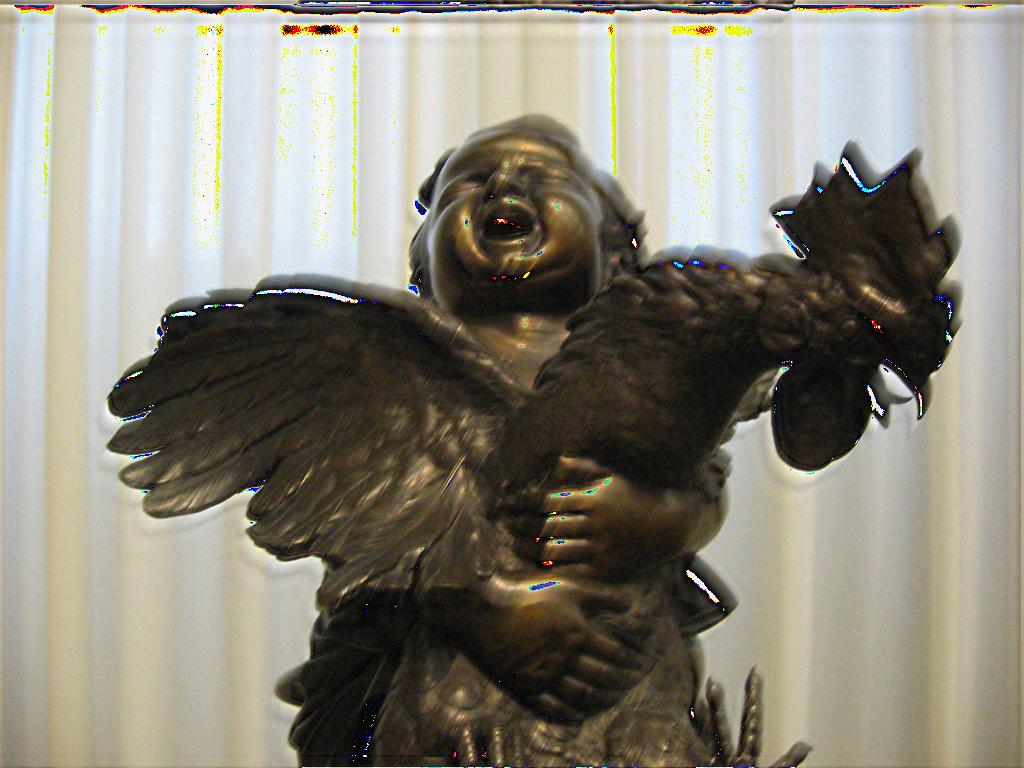
\includegraphics[width=0.2\linewidth]{../images/output/TV/boy_statue_0.001.png}}
    \hspace{1pt}
    \subfloat[]{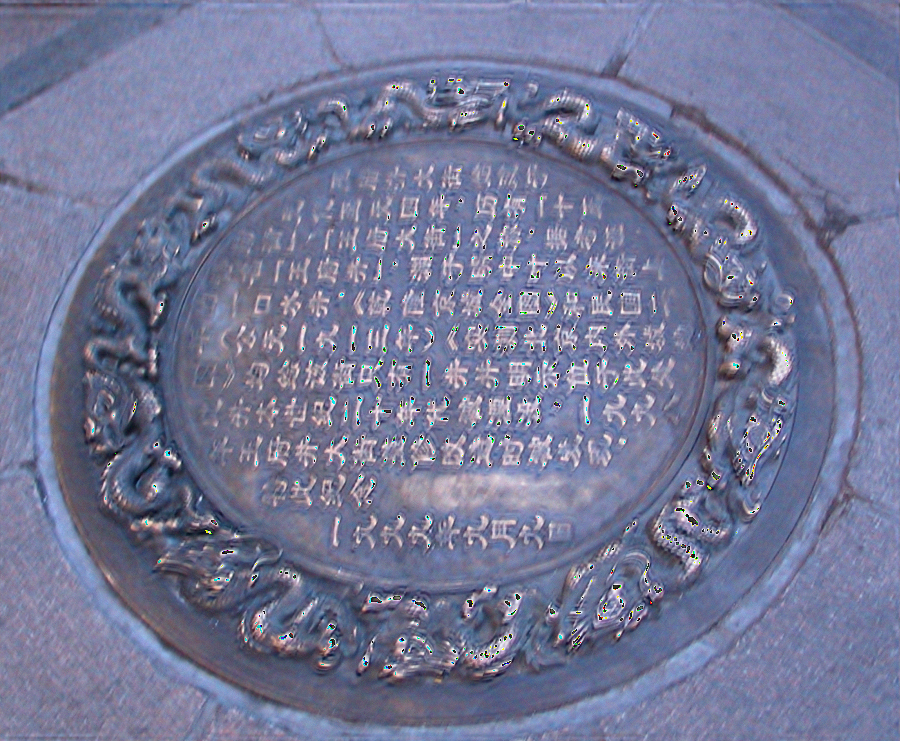
\includegraphics[width=0.2\linewidth]{../images/output/TV/hanzi_0.001.png}}
    \hspace{1pt}
    \subfloat[]{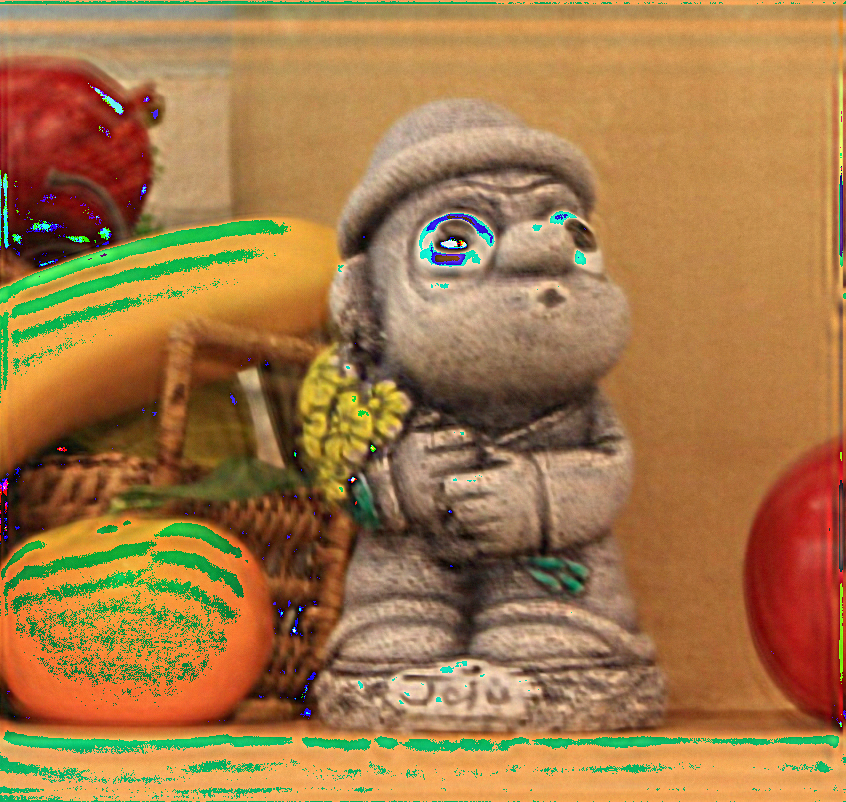
\includegraphics[width=0.2\linewidth]{../images/output/TV/harubang_0.001.png}}
    \hspace{1pt}
    \subfloat[]{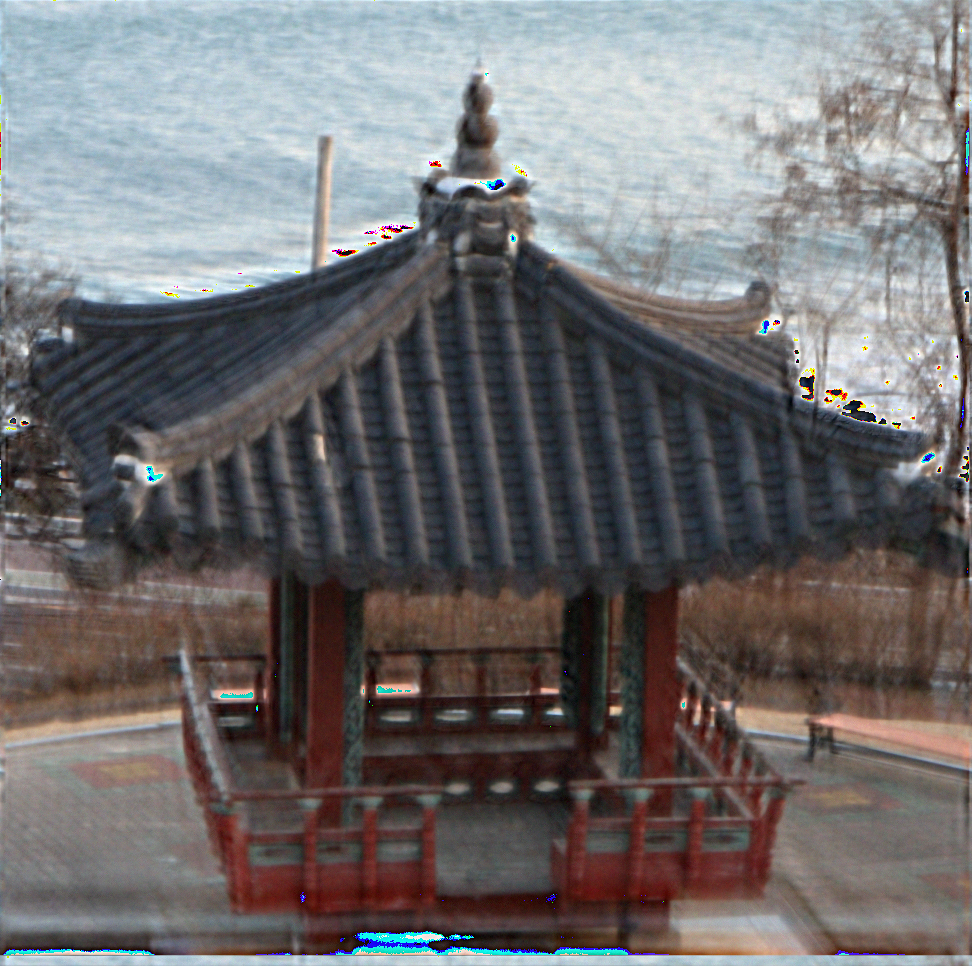
\includegraphics[width=0.2\linewidth]{../images/output/TV/summerhouse_0.001.png}}
    \caption{Result of TV Deconvolution($c$=0.001)}
\end{figure}
\begin{figure}[htbp]
    \centering
    \subfloat[]{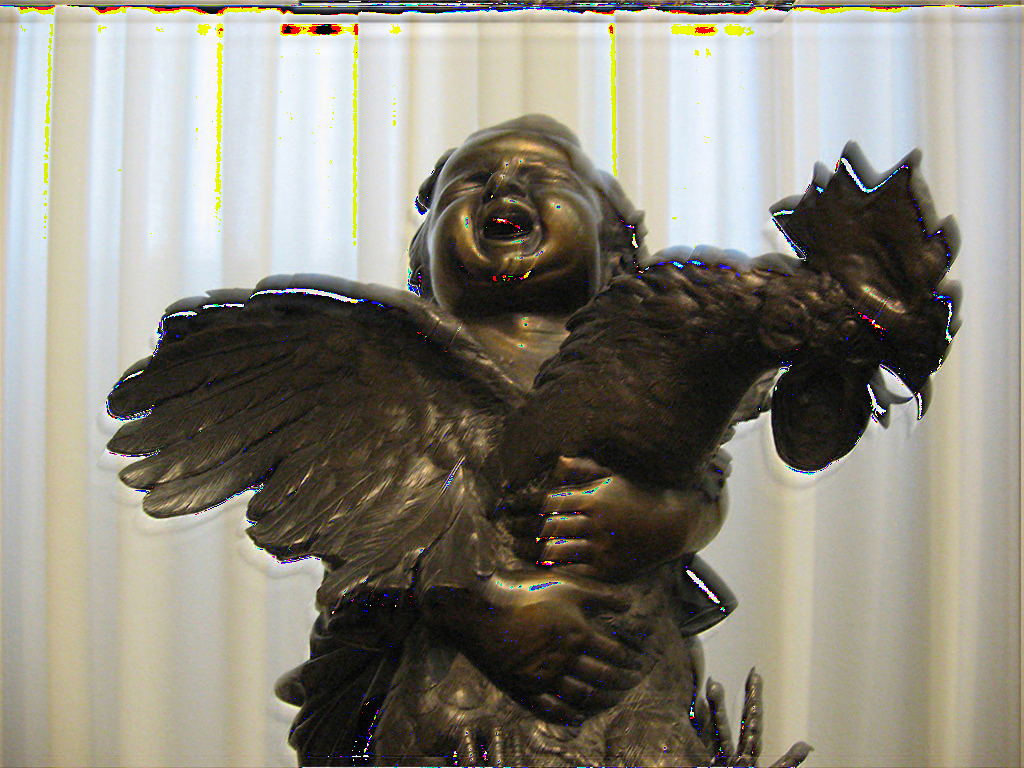
\includegraphics[width=0.2\linewidth]{../images/output/TV/boy_statue_0.0001.png}}
    \hspace{1pt}
    \subfloat[]{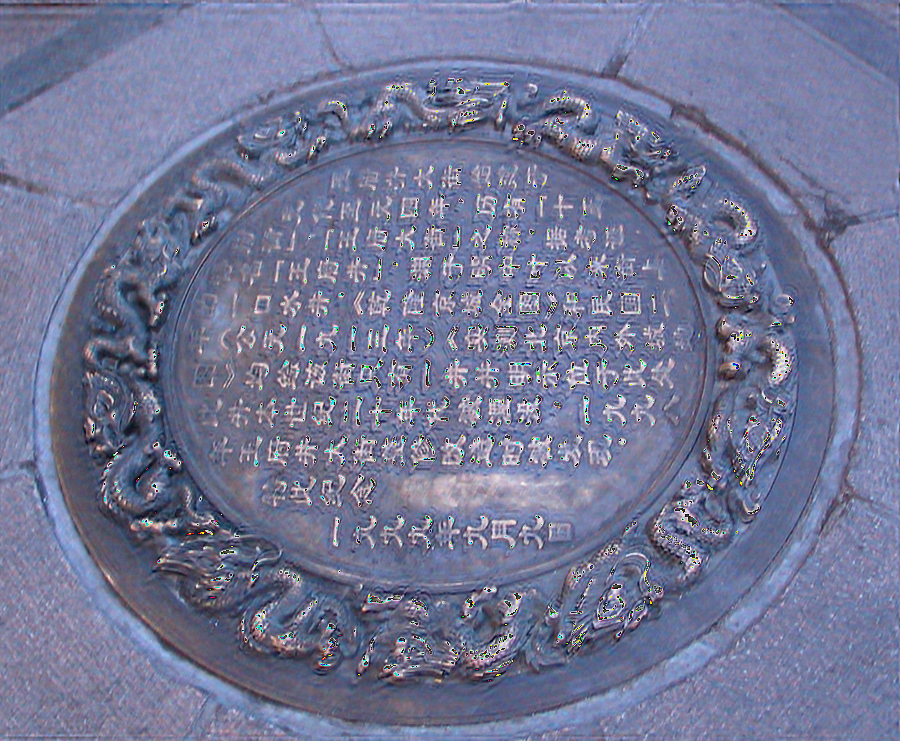
\includegraphics[width=0.2\linewidth]{../images/output/TV/hanzi_0.0001.png}}
    \hspace{1pt}
    \subfloat[]{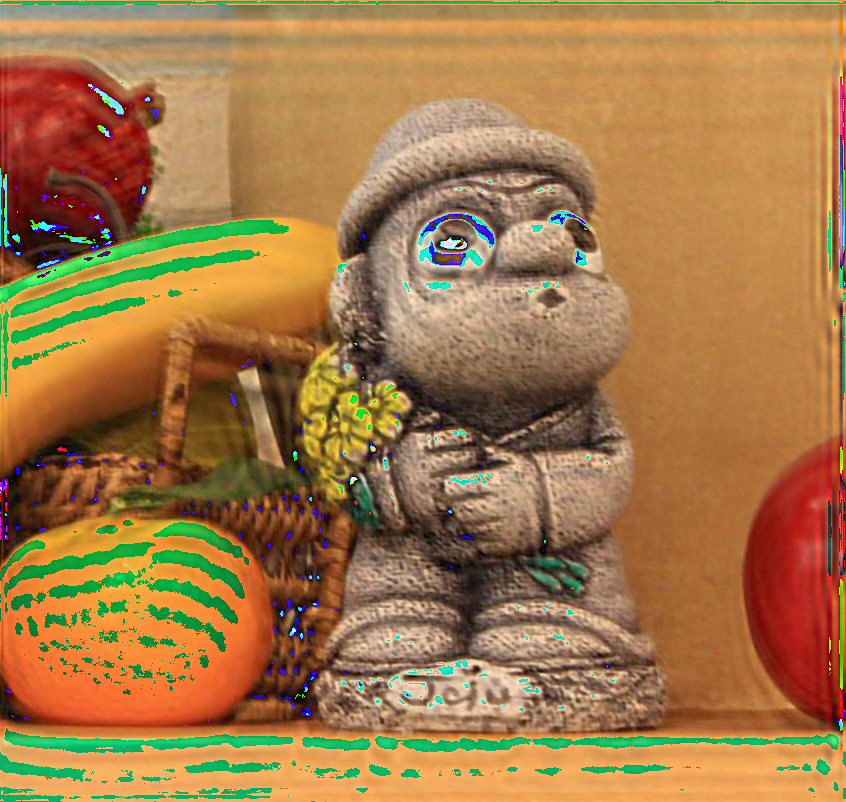
\includegraphics[width=0.2\linewidth]{../images/output/TV/harubang_0.0001.png}}
    \hspace{1pt}
    \subfloat[]{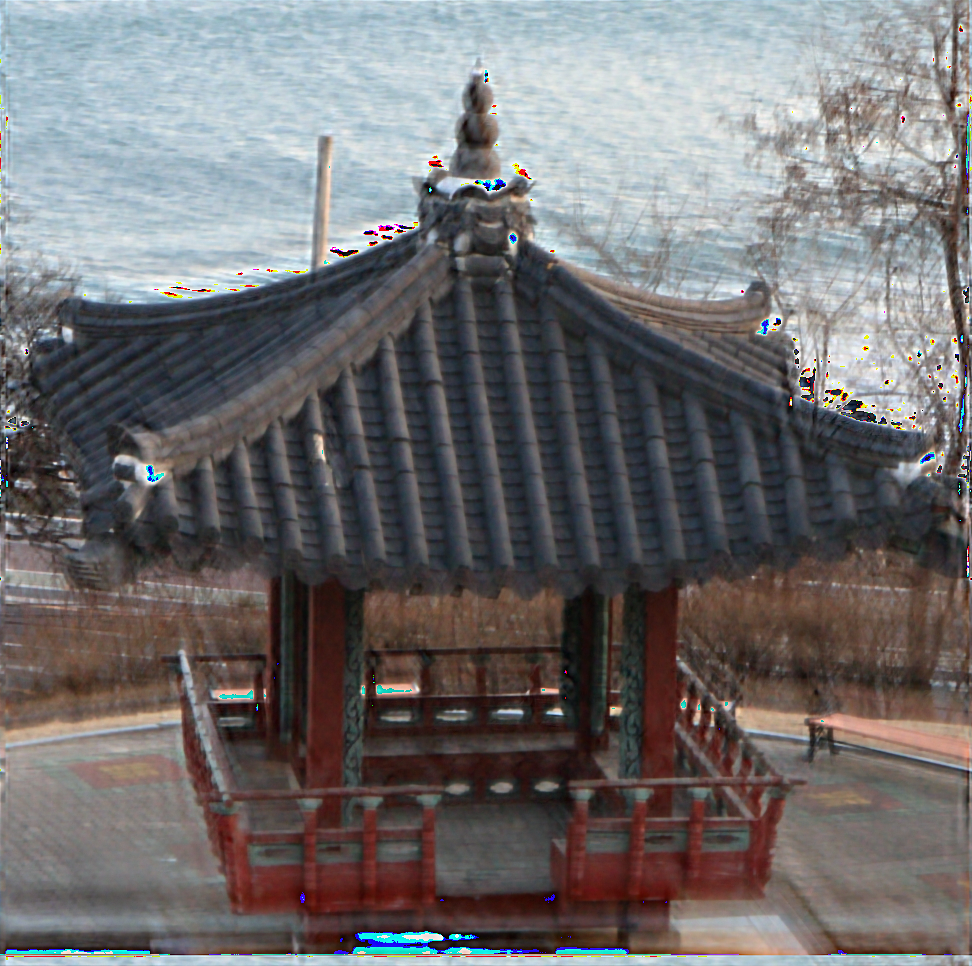
\includegraphics[width=0.2\linewidth]{../images/output/TV/summerhouse_0.0001.png}}
    \caption{Result of TV Deconvolution($c$=0.0001)}
\end{figure}

$\alpha$ 값에 따라 다른 Deconvolution 결과를 보인다.

\subsection*{Limitation}

TV Deconvolution은 Wiener Deconvolution에 비해 정교한 Deconvolution 결과를 출력할 수 있지만, 시간이 오래 걸린다는 단점이 있다.
Iteration의 수를 결정하여 적정 품질에 빠르게 도달할 수 있도록 하는 것이 중요하다고 생각된다.
또한, conjugate gradient solver의 tolerance 값과 IRLS 방법의 $\tau$ 값을 적당히 조절하여 빠른 수렴을 할 수 있도록 하는 것이 중요하다.
Non-Linear optimization을 해결하기 때문에, 빠른 optimization이 불가능하다는 단점이 있지만, Linear optimization으로의 근사가 가능하다면
속도를 더 개선시킬 수 있을 것으로 생각된다.
전체 이미지에 대한 gradient를 사용하기 때문에, downsampling한 이미지의 gradient를 이용해 원본 이미지의 gradient를 추정하는 방법 또한 유효할 것으로 생각된다.

\end{document}
